\documentclass[fleqn,10pt]{wlscirep}
\usepackage[utf8]{inputenc}
\usepackage[T1]{fontenc}
\usepackage{graphicx}
\usepackage{tablefootnote}

\makeatletter
\newcommand*{\centerfloat}{%
  \parindent \z@
  \leftskip \z@ \@plus 1fil \@minus \textwidth
  \rightskip\leftskip
  \parfillskip \z@skip}
\makeatother

\title{SUPPLEMENTARY INFORMATION: NMRlipids Databank: Overlay Databank of Lipid Membrane Simulations Arising from Open Collaboration}

\author[1]{Anne Kiirikki}
\author[2]{...}
\author[1,*]{O. H. Samuli Ollila}
%\author[1,2,+]{Christine Author}
%\author[2,+]{Derek Author}
\affil[1]{University of Helsinki, Institute of Biotechonology, Helsinki, Finland}
\affil[2]{Affiliation, department, city, postcode, country}

\affil[*]{samuli.ollila@helsinki.fi}

%\affil[+]{these authors contributed equally to this work}

%\keywords{Keyword1, Keyword2, Keyword3}

\begin{abstract}
%We present a databank of lipid bilayer simulations from the NMRlipids open collaboration project.
\end{abstract}

\begin{document}

\flushbottom
\maketitle
% * <john.hammersley@gmail.com> 2015-02-09T12:07:31.197Z:
%
%  Click the title above to edit the author information and abstract
%
\thispagestyle{empty}

%\noindent Please note: Abbreviations should be introduced at the first mention in the main text – no abbreviations lists. Suggested structure of main text (not enforced) is provided below.

\pagebreak
\section{Dependence of form factor and order parameters in the size of simulation}

\begin{figure}[!h]
    \centerfloat
    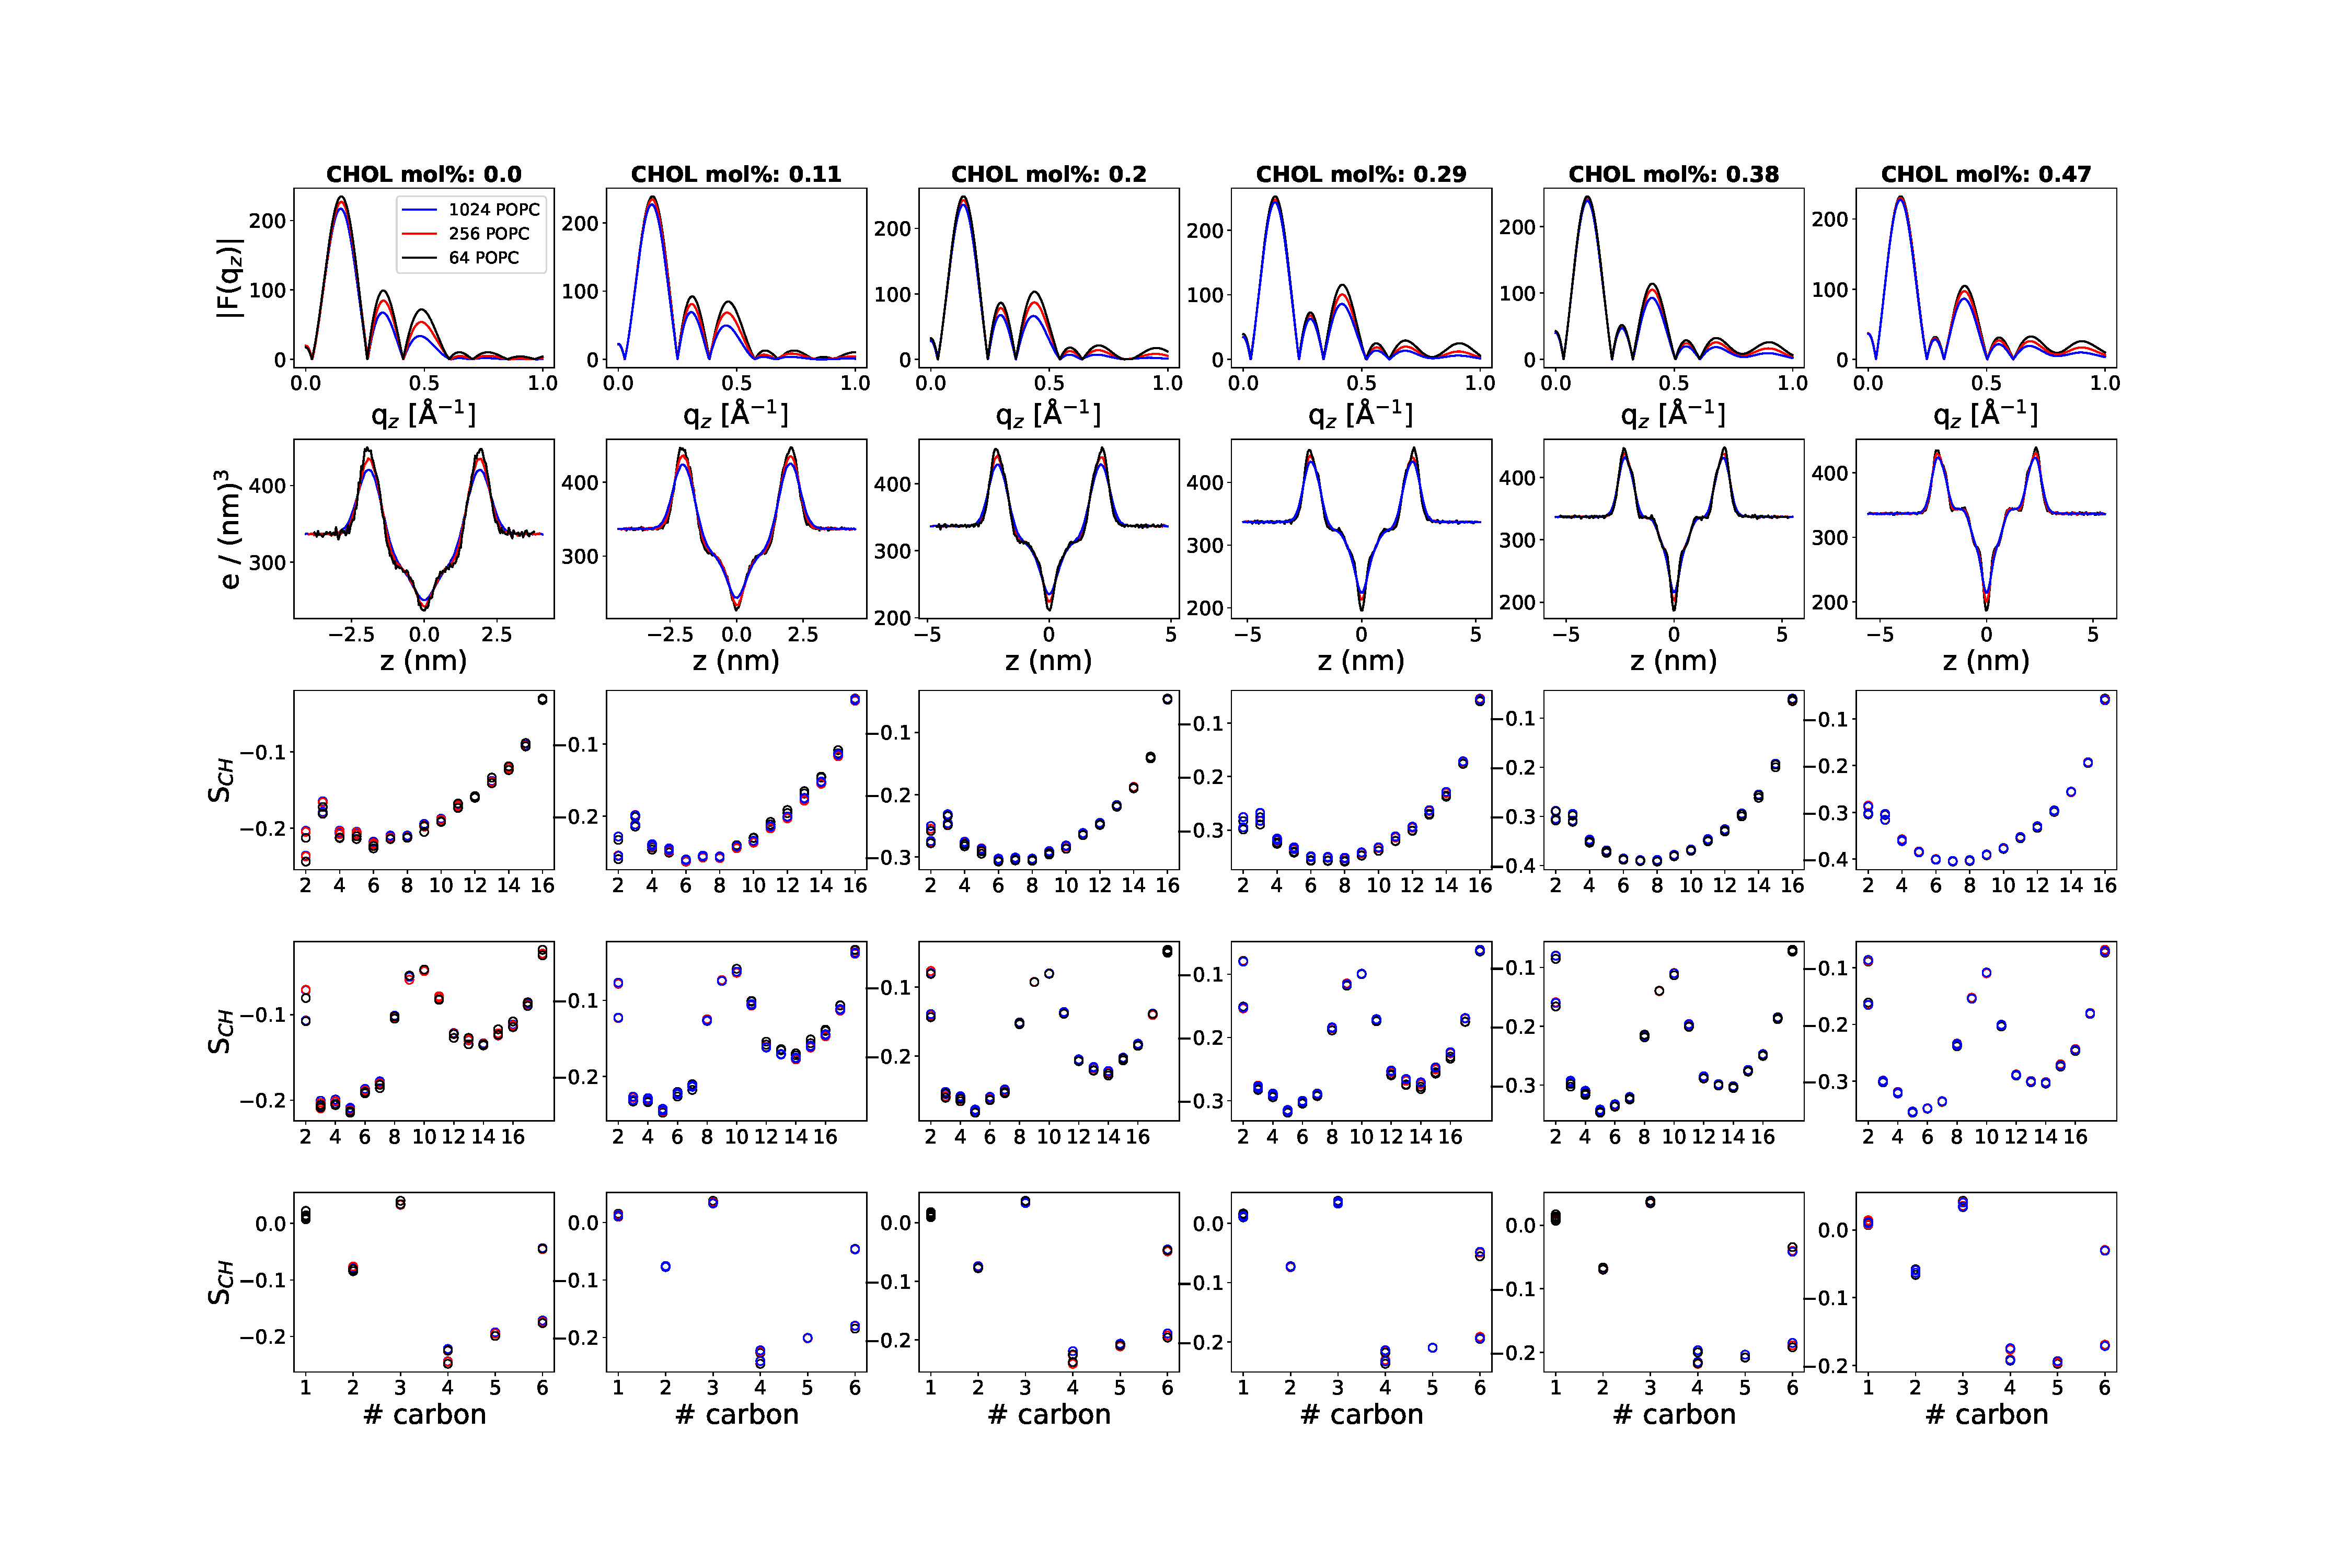
\includegraphics[width = 240mm]{Figures/SizeDependence.pdf}
    \caption{Dependence of form factor, electron density profiles along membrane normal, and C-H bond orderparameters (from top to bottom) on simulation box size with different cholesterol concentration. }
    \label{fig:sizedependence}
\end{figure}


\pagebreak
\section{Water permeation through membranes}

\begin{figure}[!h]
    \centering
    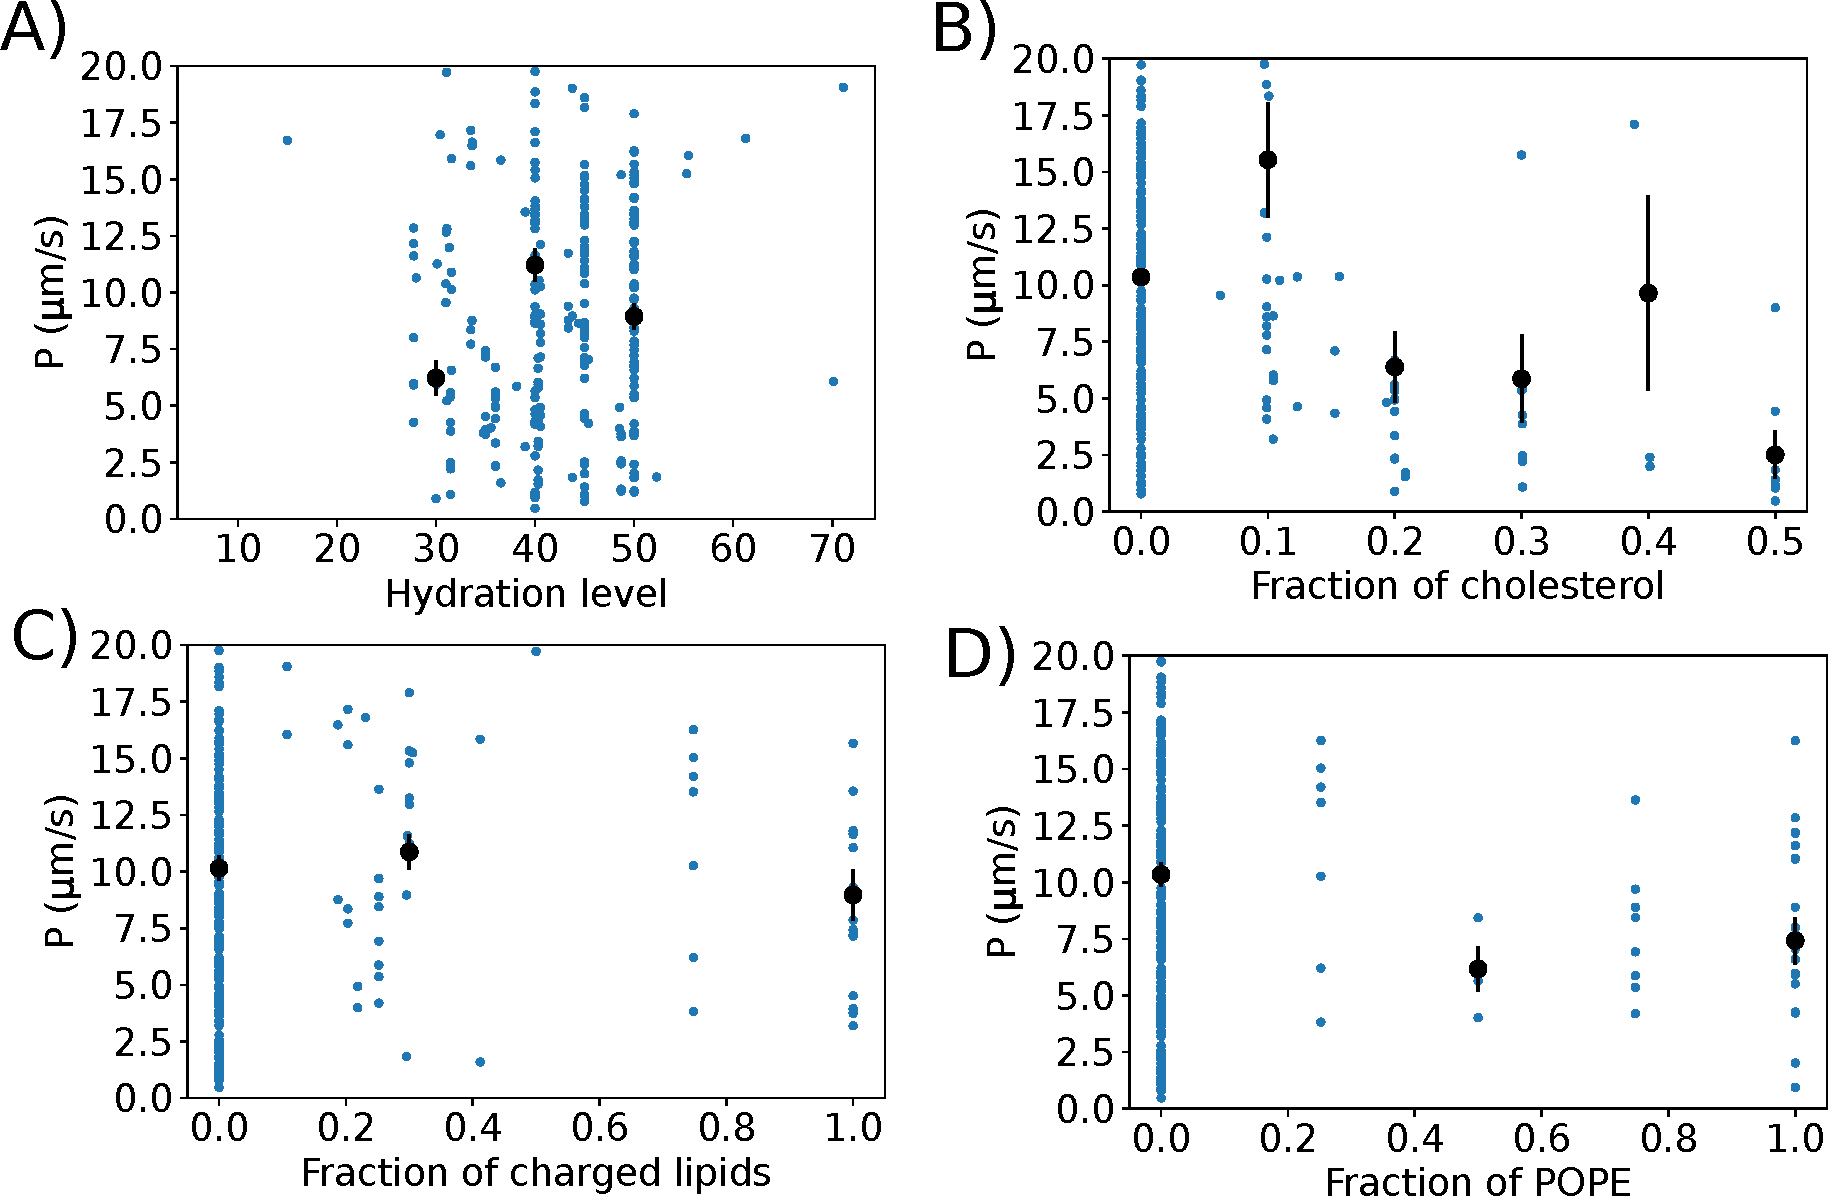
\includegraphics[width = 180mm]{Figures/permeationSI.pdf}
    \caption{a) Structure of an overlay databank. 
    More detailed structure of the layer 2 in the NMRlipids databank is illustrated in Fig.~\ref{DatabankStructure} in the SI.
    b) Distribution of the lengths of the trajectories, total number of trajectories and total lenght of the simulations in the NMRlipids databank.
    c) Distribution of lipids present in the trajectories in the NMRlipids databank. Lipids occuring in five or less simulations ('others') are listed in the right. 
    d) Currently available binary mixtures in the NMRlipids databank. 
    e) Distribution of force fields in the simulations in the NMRlipids databank.
    The figures and numbers are created on 9th of May 2022.}
    \label{fig:overlay}
\end{figure}

\pagebreak
\section{Water diffusion along membranes}

\begin{figure}[!h]
    \centering
    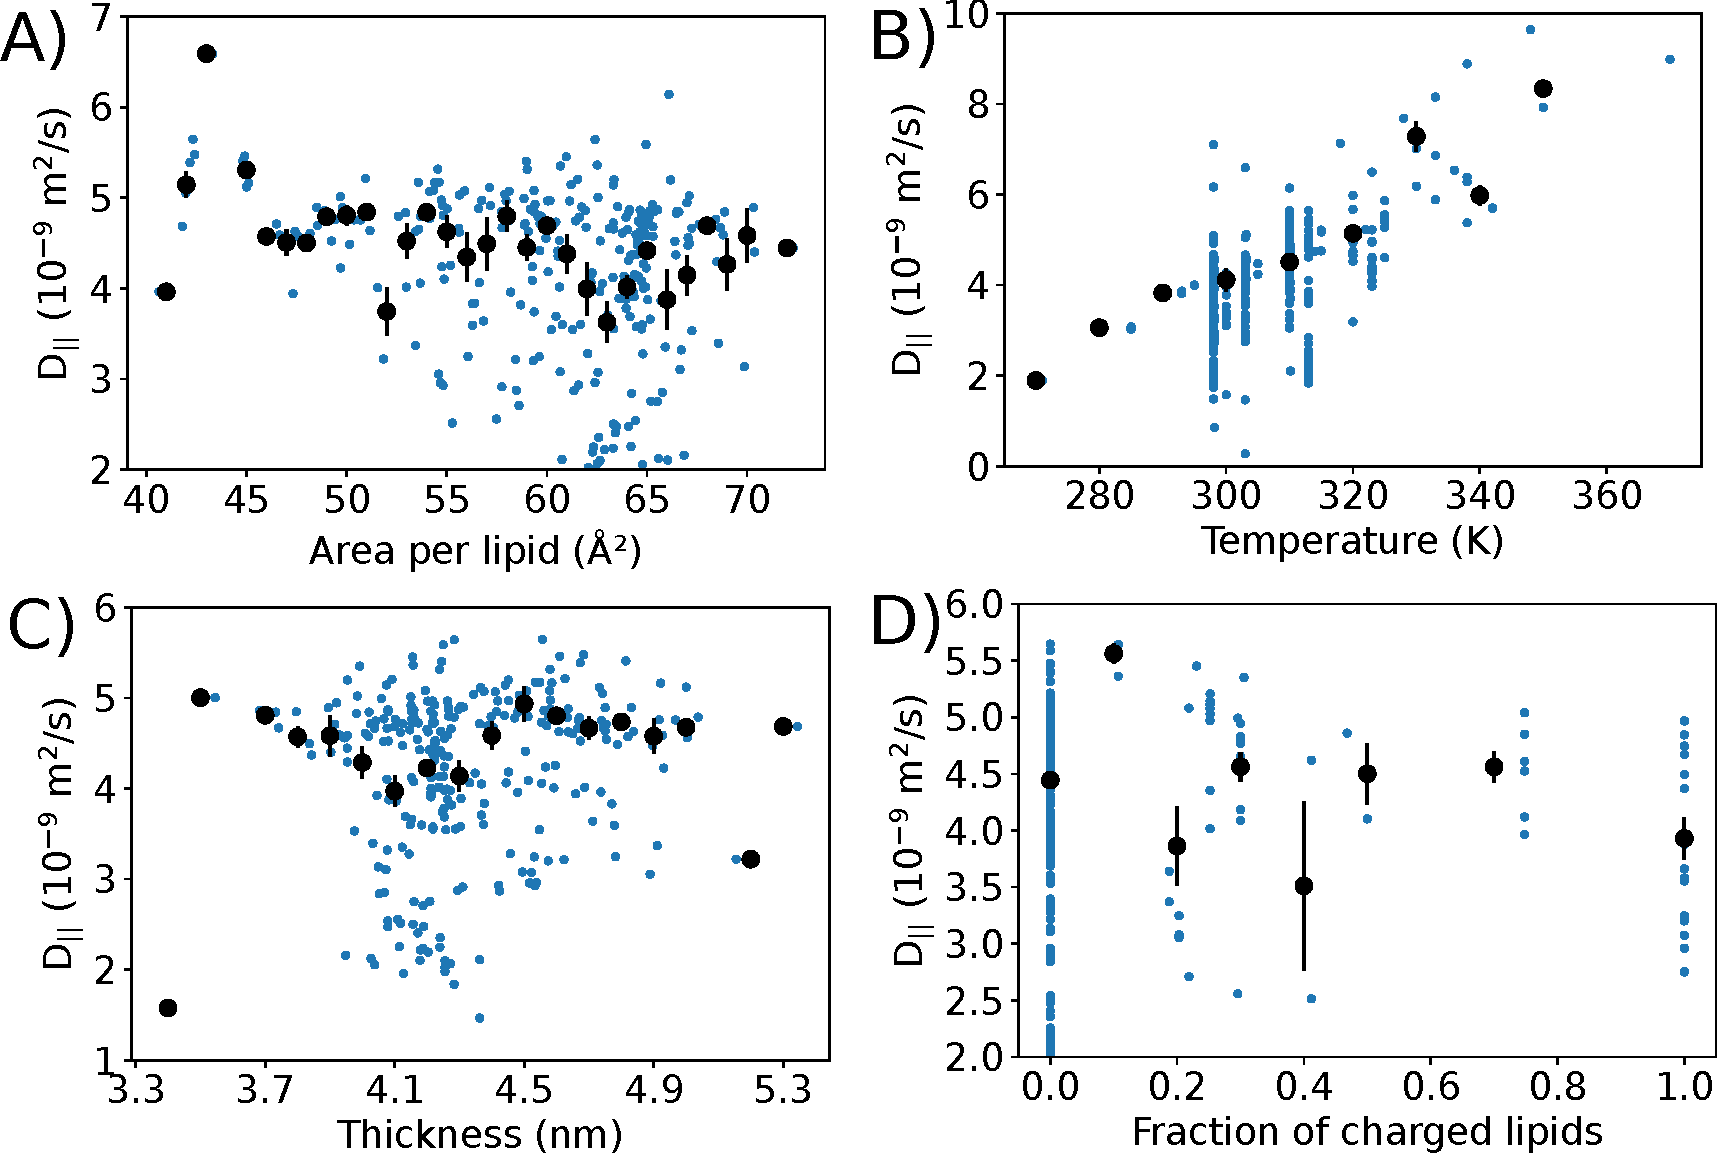
\includegraphics[width = 180mm]{Figures/LateralDiffusionSI.pdf}
    \caption{a) Structure of an overlay databank. 
    More detailed structure of the layer 2 in the NMRlipids databank is illustrated in Fig.~\ref{DatabankStructure} in the SI.
    b) Distribution of the lengths of the trajectories, total number of trajectories and total lenght of the simulations in the NMRlipids databank.
    c) Distribution of lipids present in the trajectories in the NMRlipids databank. Lipids occuring in five or less simulations ('others') are listed in the right. 
    d) Currently available binary mixtures in the NMRlipids databank. 
    e) Distribution of force fields in the simulations in the NMRlipids databank.
    The figures and numbers are created on 9th of May 2022.}
    \label{fig:overlay}
\end{figure}


\bibliography{refs.bib}

%\noindent LaTeX formats citations and references automatically using the bibliography records in your .bib file, which you can edit via the project menu. Use the cite command for an inline citation, e.g.  \cite{Hao:gidmaps:2014}.

%For data citations of datasets uploaded to e.g. \emph{figshare}, please use the \verb|howpublished| option in the bib entry to specify the platform and the link, as in the \verb|Hao:gidmaps:2014| example in the sample bibliography file.

%\section*{Acknowledgements}

%Acknowledgements should be brief, and should not include thanks to anonymous referees and editors, or effusive comments. Grant or contribution numbers may be acknowledged.

%\section*{Author contributions statement}

%Must include all authors, identified by initials, for example:
%A.A. conceived the experiment(s),  A.A. and B.A. conducted the experiment(s), C.A. and D.A. analysed the results.  All authors reviewed the manuscript. 

%\section*{Additional information}

%To include, in this order: \textbf{Accession codes} (where applicable); \textbf{Competing interests} (mandatory statement). 

%The corresponding author is responsible for submitting a \href{http://www.nature.com/srep/policies/index.html#competing}{competing interests statement} on behalf of all authors of the paper. This statement must be included in the submitted article file.

%\begin{figure}[ht]
%\centering
%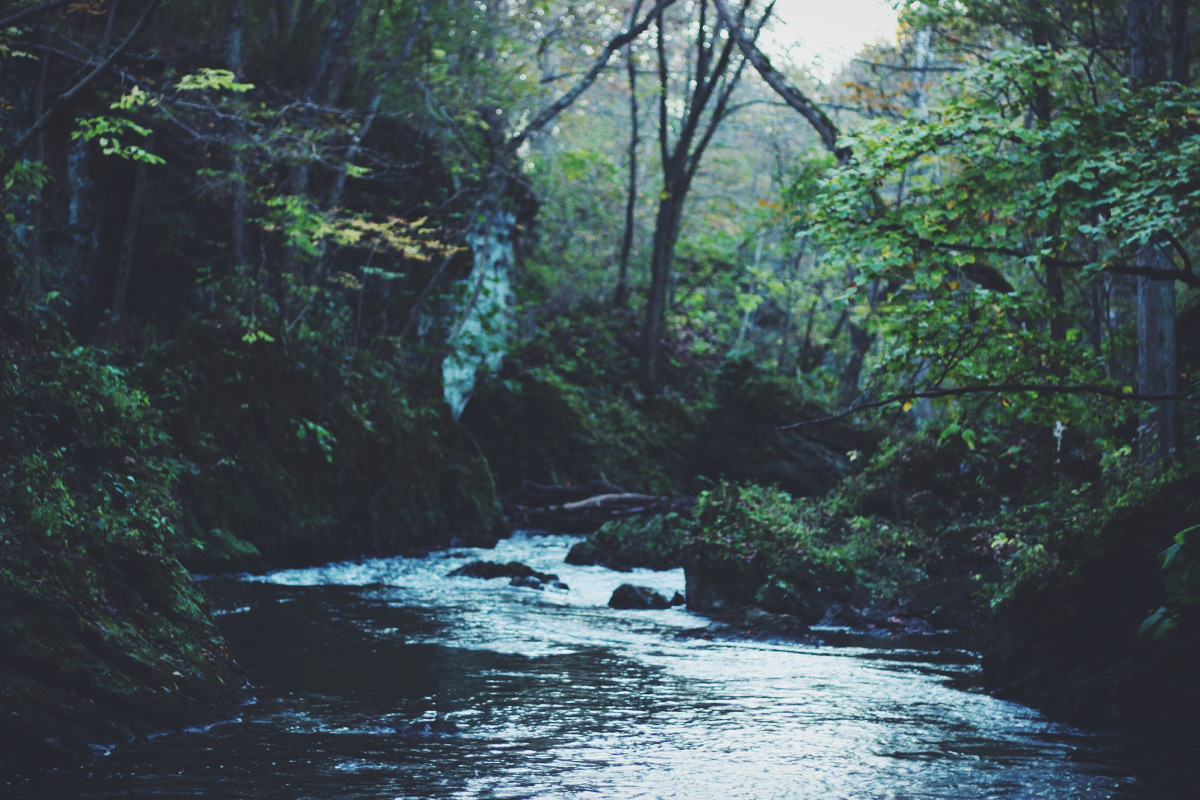
\includegraphics[width=\linewidth]{stream}
%%\caption{Legend (350 words max). Example legend text.}
%\label{fig:stream}
%\end{figure}

%\begin{table}[ht]
%\centering
%\begin{tabular}{|l|l|l|}
%\hline
%Condition & n & p \\
%\hline
%A & 5 & 0.1 \\
%\hline
%B & 10 & 0.01 \\
%\hline
%\end{tabular}
%\caption{\label{tab:example}Legend (350 words max). Example legend text.}
%\end{table}

%Figures and tables can be referenced in LaTeX using the ref command, e.g. Figure \ref{fig:stream} and Table \ref{tab:example}.

\end{document}
